\documentclass[10pt, journal,onecolumn]{IEEEtran}
\usepackage{cite}
\usepackage{graphicx}
\graphicspath{{figure/}}
\usepackage{array}
\usepackage{subfigure}
\usepackage{stfloats}
\usepackage{url}
\usepackage{nicefrac}
\usepackage{amssymb}
\usepackage{amsmath}
%\interdisplaylinepenalty=2500
\usepackage{amsfonts}
\usepackage{amssymb}
\usepackage{booktabs}
\usepackage{relsize}
\usepackage[pdfpagelabels]{hyperref}
\usepackage{float}
\usepackage[round]{natbib}
\usepackage{color}
\usepackage{authblk}
\usepackage{caption}
\newcommand{\ra}[1]{\renewcommand{\arraystretch}{#1}}

% Allow paragraph indents inside lists.
\usepackage{enumitem}
\setenumerate{listparindent=\parindent}

%\usepackage{kbordermatrix}

\hypersetup{
  colorlinks   = true, %Colours links instead of ugly boxes
  urlcolor     = blue, %Colour for external hyperlinks
  linkcolor    = blue, %Colour of internal links
  citecolor   = red %Colour of citations
}

\floatstyle{ruled}
\newfloat{algorithm}{tbp}{loa}
\floatname{algorithm}{Algorithm}

\newtheorem{theorem}{Theorem}
\newtheorem{corollary}{Corollary}
\newtheorem{proposition}{Proposition}
\newtheorem{definition}{Definition}
\newtheorem{lemma}{Lemma}

\newcommand{\norm}[1]{\left\lVert#1\right\rVert}
\newcommand{\abs}[1]{\left\lvert#1\right\rvert}
\newcommand{\inner}[1]{\left\langle#1\right\rangle}
\def\b#1{\mathbf{#1}}
\def\t#1{\text{#1}}


\title{Predicting the 2014 Ebola Outbreak in West Africa using Network Analysis \\
       {\large Milestone Report} }

\author{Shafi Bashar, Mike Percy, Romit  Singhai}
\affil{\textit {\{shafiab, mp81, romit\}@stanford.edu}}

\renewcommand\Authands{ and }


\begin{document}

\maketitle

\begin{abstract}
The current Ebola outbreak in West Africa is the worst in history.
Most traditional epidemiological models are compartmental models that have a random-mixing
assumption. These models calculate the
effective reproductive rate of an outbreak. We survey three of these models: the classic
SIR (Susceptible, Infectious, Recovered) model and two extensions used in Ebola research.

Network models allow for avoiding the random-mixing
assumption inherent in compartmental models.
This is done by assigning each individual a finite set of permanent contacts.
We review generated contact network models for SARS, including an urban network, a random network, and
a scale-free network.
We then review a worldwide network model that represents traffic flowing across transportation
networks and consider approaches for predicting the extent of an Ebola outbreak.

\end{abstract}



%%%%%%%%%%%%%%%%%%%%%%%%%%%%%%%%%%%%%%%%%%%%%%%%%%%%%%%%%%%%

\section{Introduction}
\label{sec:Introduction}

TODO: Add introduction



%%%%%%%%%%%%%%%%%%%%%%%%%%%%%%%%%%%%%%%%%%%%%%%%%%%%%%%%%%%%

\section{Related Work}
\label{sec:RelatedWork}

Related work by \citep{gomes2014assessing} attempts to predict the spread of Ebola
to different parts of the world based on a model that incorporates both the compartmental
approach and the use of world-wide air traffic flows.

In \citep{meyers2005network}, the authors model the spread of the 2002-2003
outbreak of SARS in Hong Kong and Canada using a contact network.
A contact network model attempts to characterize every interpersonal contact that can
potentially lead to disease transmission in the community, with each person in the
community represented as a node and each contact represented as an edge between them.

\label{SubSec:SIR}

The majority of research in epidemiological theory is based on the compartmental model,
which is not a network model.
In order to simply capture the dynamics of disease spread over time, the compartmental model
employs a a population-wide random mixing assumption, meaning that each individual has a
small and equal chance of coming into contact with any other individual in the population. 
To model the progress of an epidemic in a large population, the
individuals in the population are compartmentalized according to the state of the disease. The most
widely used such model is the SIR model introduced in \citep{very_old_paper}:

\begin{itemize}
\item \textbf{Susceptible (S):} Individuals who have not yet caught the disease from contact with an infectious
  individual.
\item \textbf{Infectious (I):} Individuals who have the disease. They have some probability of
  infecting susceptible people.
\item \textbf{Recovered (R):} Individuals who have experienced the full infectious period, and are
  now non-infectious and immune.
\end{itemize}

The changes among these states over time are represented by a set of differential equations.
The basic reproductive number $R_0$
is defined as the average number of secondary cases generated by a primary case in a pool of mostly
susceptible individuals, and is an estimate of epidemic growth at the start of an outbreak if
everyone is susceptible.

\label{SubSec:SEIR}

In \citep{chowell2004basic}, the authors model the effect of Ebola outbreaks in 1995 in Congo and in
2000 in Uganda using a compartmental model similar to the SIR model. However,
a distinct feature of Ebola is that individuals exposed to the virus who become infectious do so
after a mean incubation period. In order to reflect this feature, in the SIR model is extended with
an additional ``Exposed'' compartment state. This SEIR model is summarized in
Figure \ref{fig:SEIR_model}:

\begin{figure}[h!]
\captionsetup{justification=centering}
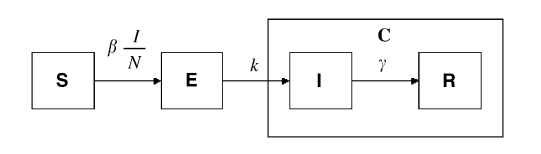
\includegraphics[scale=0.4]{seir_model_fig}
\centering\caption{SEIR model}
\label{fig:SEIR_model}
\end{figure}

\label{SubSec:SEIHFR}

In \citep{legrand2007understanding}, the Ebola outbreaks in Congo in 1995 and Uganda in 2000
are also studied. However, a major difference from
\citep{chowell2004basic} is that \citep{legrand2007understanding} models the spreading of disease
in heterogeneous settings. In order to gain better insight of the epidemic dynamics,
the infectious phase is subdivided into three stages:
infection in a community setting (I), infection in a hospital setting (H), and
infection after death assuming a traditional funeral (F).

This SEIHFR compartmental model is summarized in Figure \ref{fig:SEIHFR_model}.

\begin{figure}[h!]
\centering
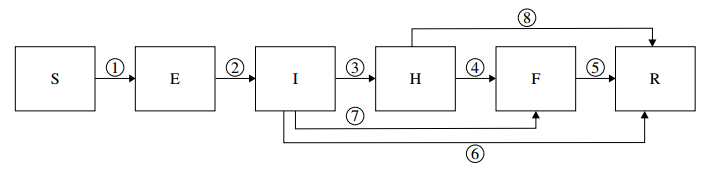
\includegraphics[scale=0.5]{seihfr_model_fig}
\caption{SEIHFR model}
\label{fig:SEIHFR_model}
\end{figure}

For our purposes, as described below, we stopped short of implementing this complicated model.

\bigskip




%%%%%%%%%%%%%%%%%%%%%%%%%%%%%%%%%%%%%%%%%%%%%%%%%%%%%%%%%%%%

\section{Modeling localized epidemic spread}
\label{sec:IntraCountry}




%%%%%%%%%%%%%%%%%%%%%%%%%%%%%%%%%%%%%%%%%%%%%%%%%%%%%%%%%%%%

\subsection*{\textbf{Estimating model parameters and basic reproduction number for 2014 Ebola data using a random mixing model}}

In first phase of the project, to calculate the basic reproduction number of the current Ebola epidemic spread at different countries, we performed model fitting on the data we gathered from \cite{cmriversdata}. We considered the SEIR model described in \cite{chowell2004basic}. The SEIR model under consideration is a non-linear model with six parameters. The current Ebola epidemic is still spreading and depending on the preventative measures  taken, the underlying dynamics of the spread can change drastically anytime. We fitted our model to three countries in the West Africa - Guinea, Sierra Leone and Liberia. In addition, we performed model fitting for the West Africa Region by adding up the data from these three countries. Given the limited number of data available, instead of fitting all six parameters to the model, we decided to fix some of the parameters based on the studies on previous Ebola epidemic. In \cite{chowell2004basic}, the incubation time of the Ebola $1/k$ is found to be varying between 1 to 21 days, with a mean time of 6.3 days for previous Ebola spread. For ease of data fitting, we set this parameter value to the mean value of 6.3 days. We note that, the dynamics of the current epidemic may differ from previous one, and therefore fixing a value based on the prior estimate may lead to some inaccuracy. To model the effect the intervention on the spread of the epidemic, a modified transmission rate $\beta_1$ is generally used instead of the initial transmission rate $\beta_0$ at later stage of the epidemic. The transition of $\beta_0$ to $\beta_1$ depends on intervention time $\tau$ and decaying factor $q$. The choice of intervention time is a very difficult problem. To this end, we looked into different sources like Wikipedia, WHO and CDC website to learn more about the timeline of the spread. In Guinea, a 2-year-old boy fell in December 2, 2013, later diagnosed as Ebola patient. We consider this incidence as the index case for Guinea and set $t_0$ to December 2. In March 2, the Government of Guinea informed WHO regarding the possibility of Ebola epidemic and declared national heath emergency. We considered this date as the intervention date and set $\tau$ to 110. In Sierra Leone, one person fell in April 2014. In June 12, 2014 the country declared emergency and closed borders with neighboring Guinea and Liberia. We consider the first date as $t_0$ and second date as intervention time, therefore set $\tau$ to 50. In Liberia, in March 31, 2014, there were official confirmation of two person getting infected from Ebola. We set this date to $t_0$ and set $I_0$ and $C_0$ in our model as 2. The Government of Liberia shut down all schools in July 30, 2014. We consider this date as the date of intervention and set $\tau$ to 120.

In order to fit the non-linear SEIR model to data, we used non-linear least square estimation. We use the reported data $(t_i, c_i)$ for $i=1,2,\ldots,n$ where $t_i$ denote the $i-th$ reporting time and $c_i$ as the cumulative number of infectious cases from the beginning of outbreak time $t_0$ to time $t_i$. The optimization problem contains a large number of local minimas. Therefore, the choice of initial parameter estimate is an important consideration to get the global optimum solution. In order to find a good initial choice of the parameters as an input to the non-linear least square solver, we first perform a Latin hypercube sampling on the  4-dimensional parameter space.  We grid up the hypercube with a number of grid points in each dimension.  We then choose the sample that minimizes the least square error as the initial input. In order to calculate the 95\% confidence interval of estimated parameter, we performed bootstrapping based on residual error.

\begin{figure}[ht]
\centering
\subfigure[Guinea]{
  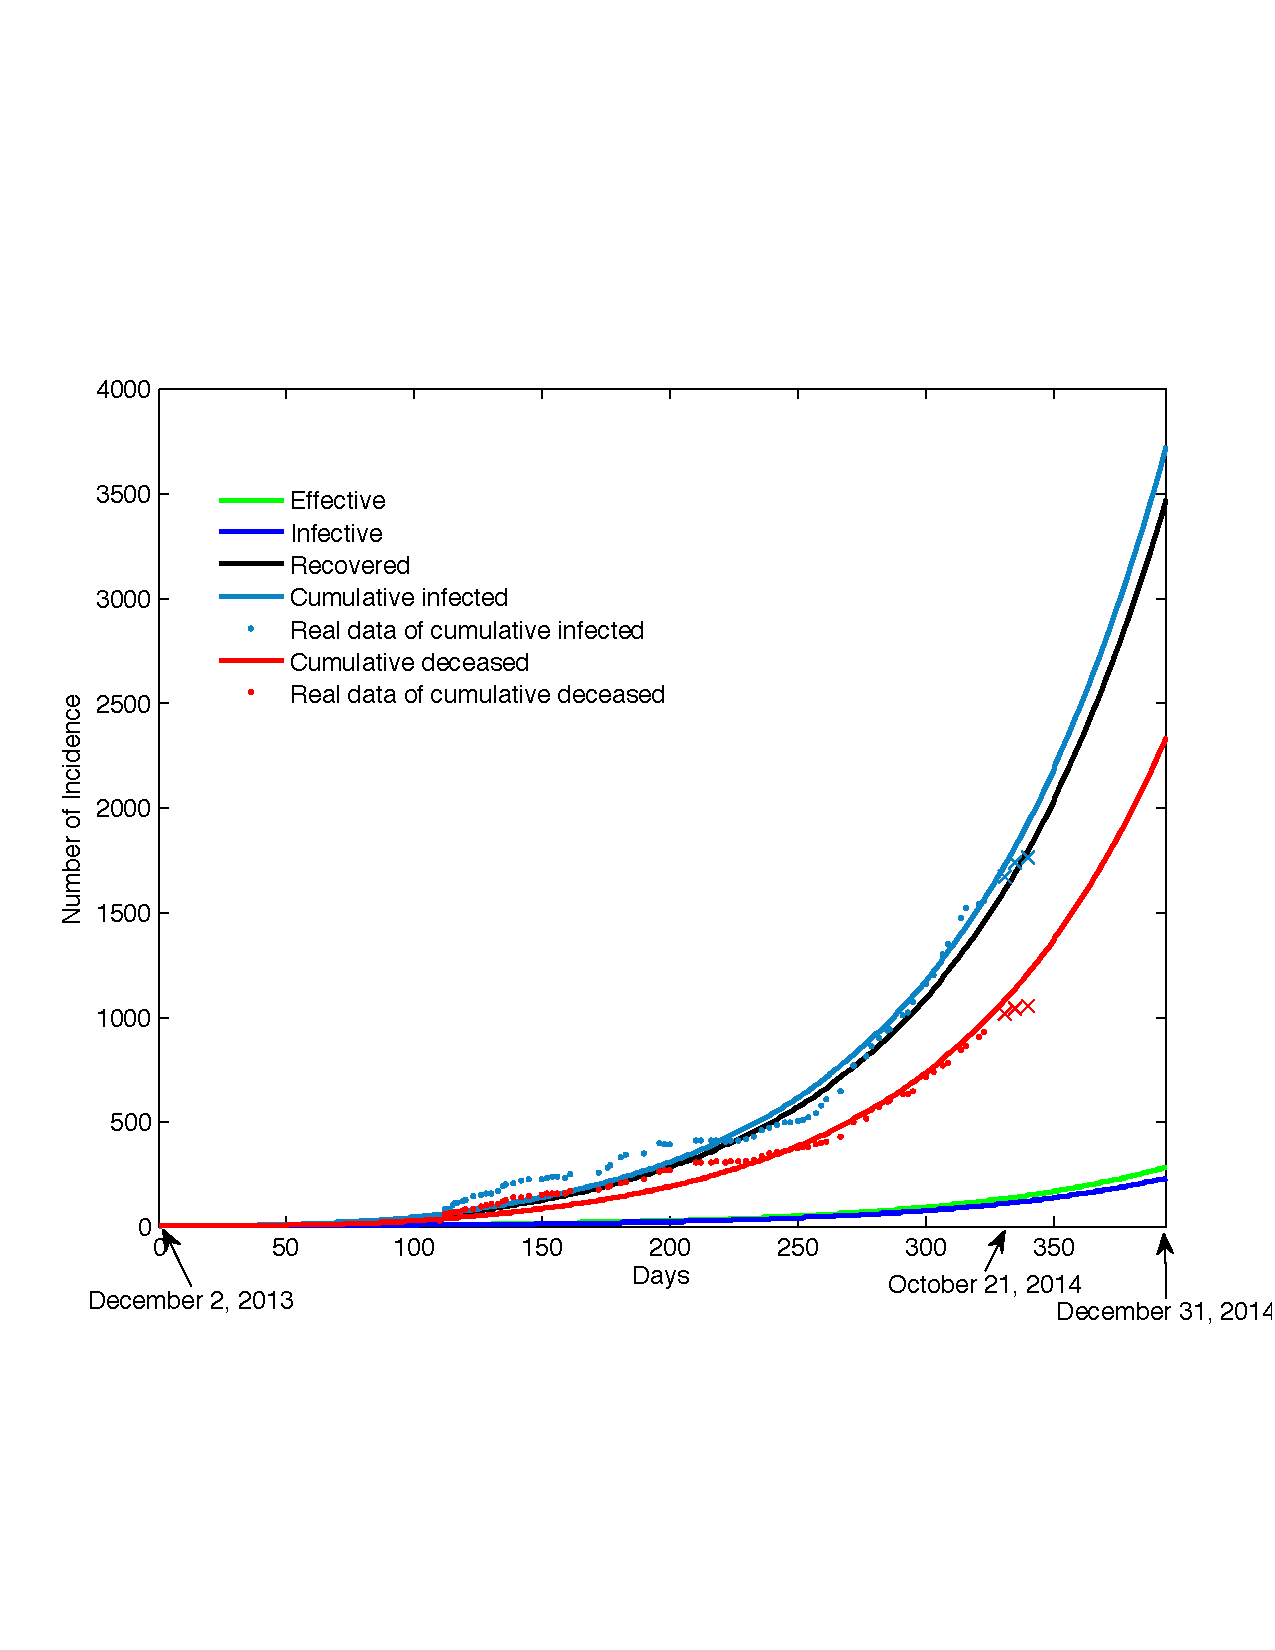
\includegraphics[width=0.47\textwidth]{Guinea.pdf}
  \label{fig:subfigure1}}
\quad
\subfigure[Sierra Leone]{
  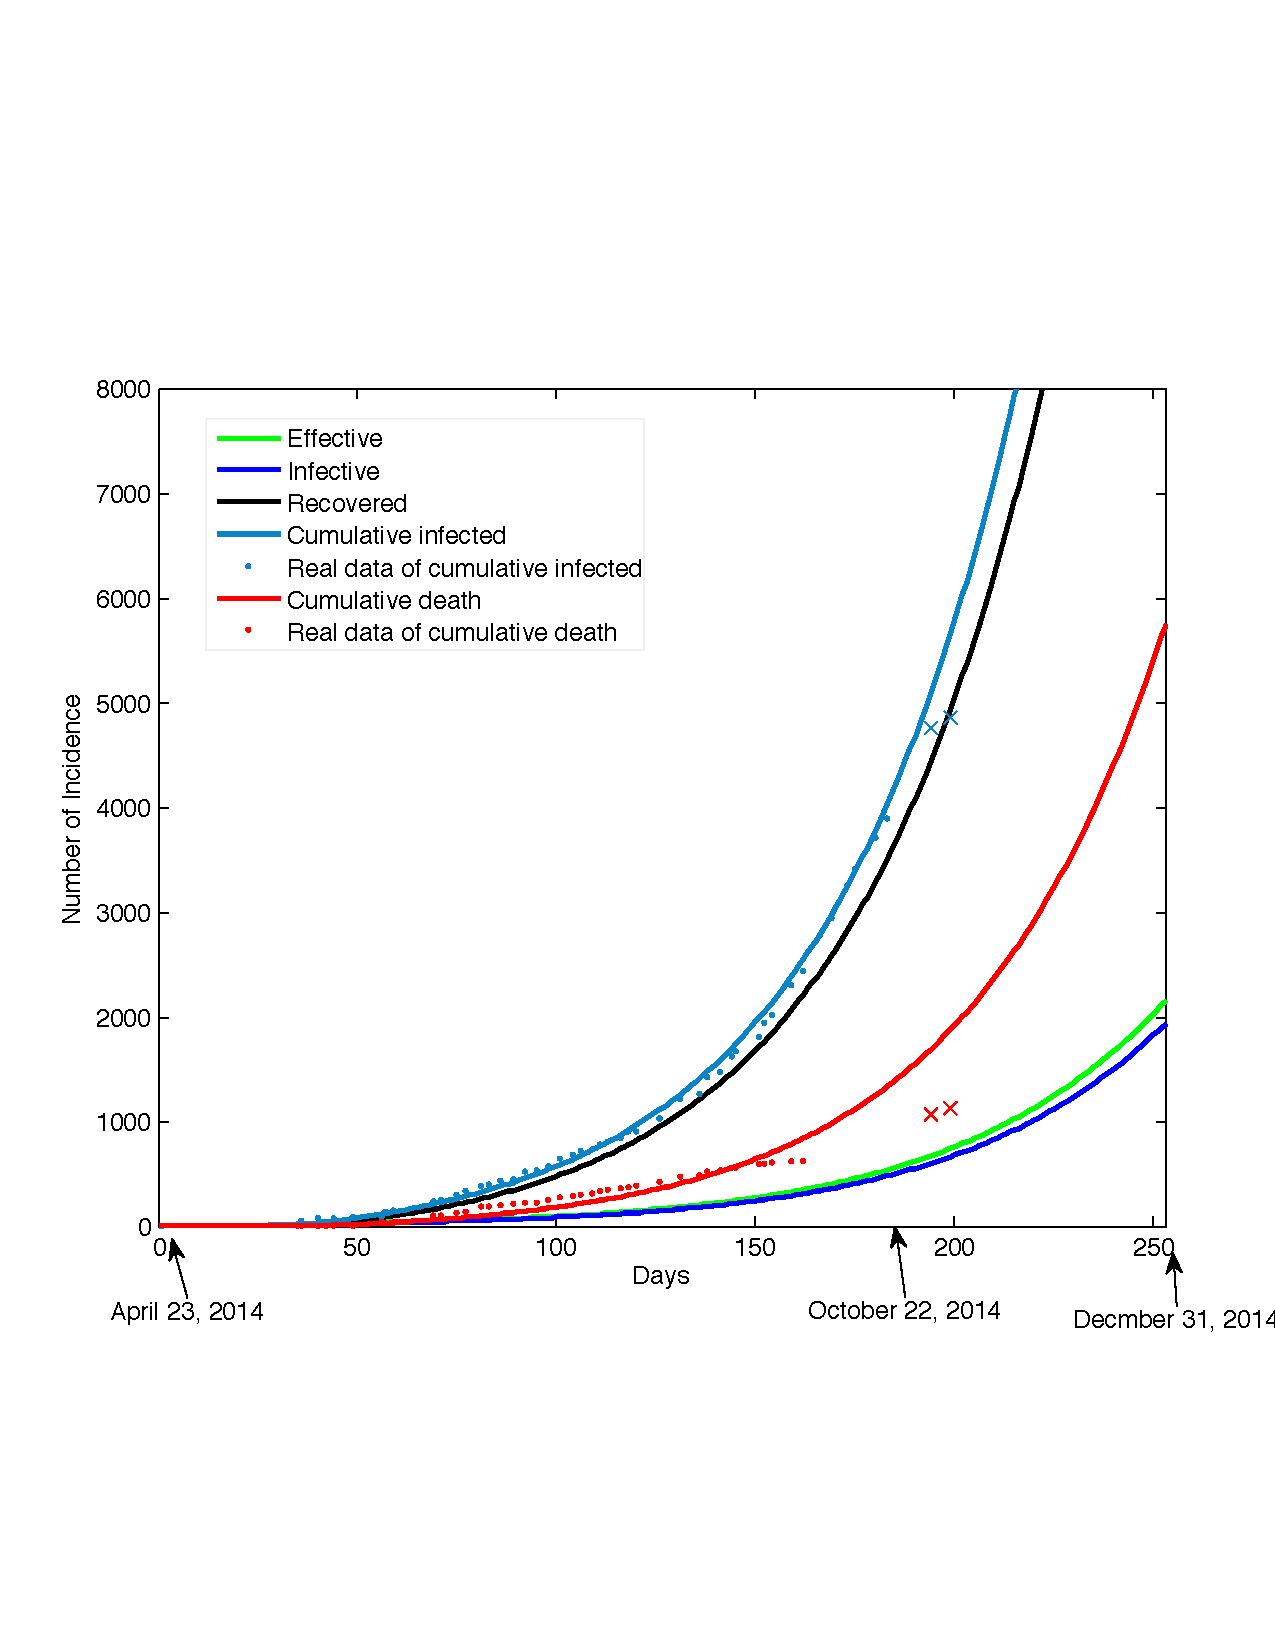
\includegraphics[width=0.47\textwidth]{SierraLeon.pdf}
  \label{fig:subfigure2}}
\subfigure[Liberia]{
  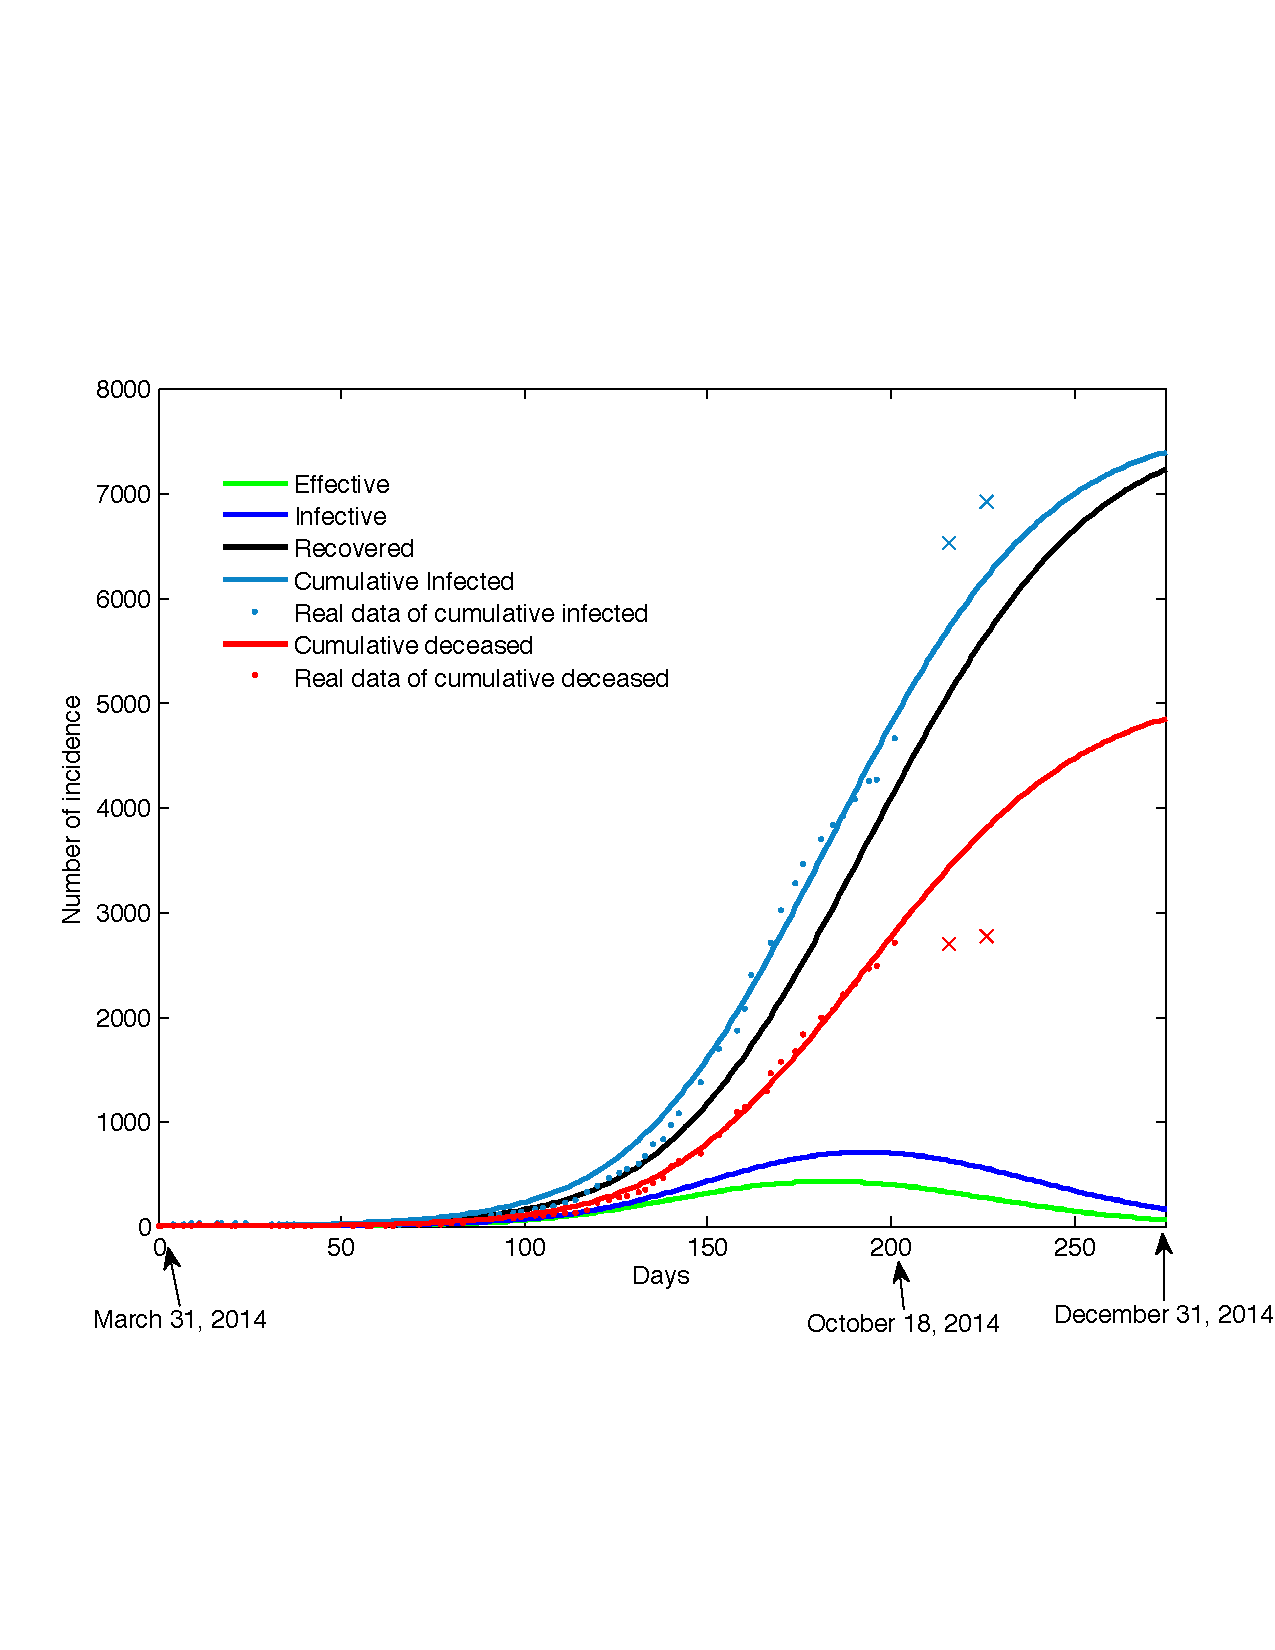
\includegraphics[width=0.47\textwidth]{Liberia.pdf}
  \label{fig:subfigure3}}
\quad
\subfigure[West Africa]{
  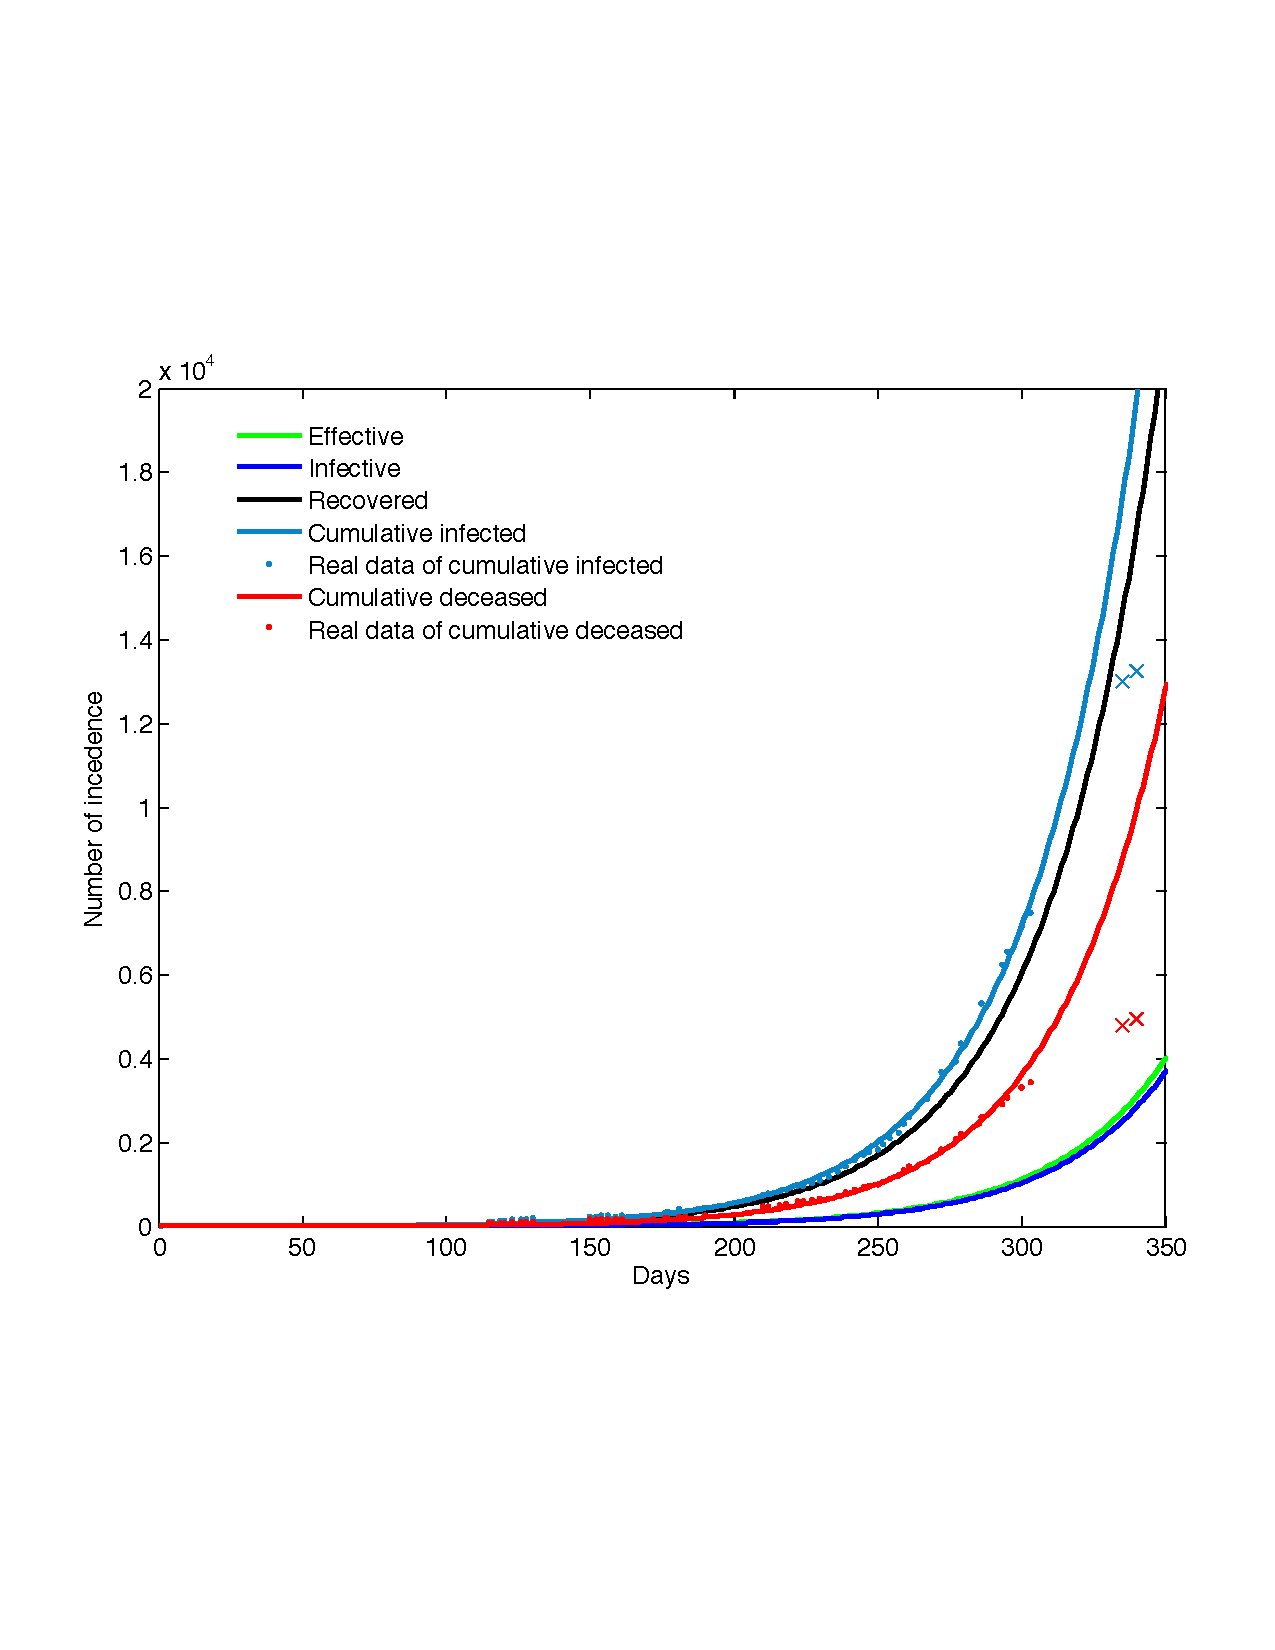
\includegraphics[width=0.47\textwidth]{WestAfrica.pdf}
  \label{fig:subfigure4}}

\caption{SEIR model fit results for 2014 Ebola epidemic data}
\label{Fig:figurePrediction}
\end{figure}


The estimated parameters for the SEIR model of Guinea, Sierra Leone, Liberia, as well as West Africa region is presented in the appendix. In Figure \ref{Fig:figurePrediction}, we presented the the number of incidence at different compartments of the SEIR model, as well as the cumulative number of infectious cases over time. Our model fit was based on the last data we collected in October 21, 2014. As of today, November 11, 2014, few additional data points are available; we also plotted those data points in the graph. In addition to that, we extrapolated the graph up to December 31, 2014. We note that, the forecasting to future cases may not be appropriate as the underlying factors of the Epidemic are changing rapidly with the increase in safety measures. We observe that, the prediction of the model to the cases up to November 11 is mostly in par with the observed data for Guinea and Sierra Leone. We note that, for Guinea epidemic, we have data for the longest range of days as the initial case was in December 2. The estimated model, therefore, captures most of the dynamics of the spread in Guinea in contrast to the other cases. In case of Liberia, our prediction under-estimated the observed data. Our guess is the estimated parameters for Libera may be overfitting the model. While performing some exploratory analysis on the Liberia data, we observed some discrepancies, e.g. decrease in cumulative value from the previous data points, which may somewhat distorted the model fitting parameters. For the West Africa region plot, our prediction number is much higher that the actual data. This is understandable, as the underlying assumption behind SEIR model is random mixing.  Within a country without any movement restriction, this model is some what appropriate. However, for the aggregated model among multiple countries, this assumption is no longer valid due to stricter movement regulations between country borders. Therefore a model with random mixing assumption will over predict the infectious number of cases.

As an extension of the above approach, for find parameters for the model based on the current data, we designed and ran the simulation using mcmc approach with input as time series data for the various infected regions.
Initial values for the various parameters were assumed as above for the prior distribution but the range based on the literature was used to find the most appropriate values for the current outbreak. For example $\beta_0$  had a range [0,1],  $\beta_1$ had a range [0,1], infection time($1/\gamma$) had range [3.5,10.7], incubation time ($1/k$) had a range [5, 22] and ($\tau$)  had a range [100,150]. The simulation is currently running on a server and we will have results in the final report.




%%%%%%%%%%%%%%%%%%%%%%%%%%%%%%%%%%%%%%%%%%%%%%%%%%%%%%%%%%%%

\subsection*{\textbf{Planned network-based modeling approaches}}

TODO: We are looking at modeling via $G(n,m)$ and contact networks.



%%%%%%%%%%%%%%%%%%%%%%%%%%%%%%%%%%%%%%%%%%%%%%%%%%%%%%%%%%%%

\section{Predicting worldwide spread}
\label{sec:Worldwide}

\subsection*{\textbf{Approach}}
In order to predict how the epidemic might spread across the world, we have assembled a
worldwide network based on international trade. Because the trade numbers are in US dollars,
we have assumed a linear relationship between exports in dollars and travelers going abroad.
This is a strong assumption, and we are currently exploring options for utilizing the trade network
in this regard.

\subsection*{\textbf{Data Preparation}}

The trade network dataset we are using is based on data retrieved from the web service API to the
UN Comtrade database \citep{uncomtradedata} via their web service API.
The data queried for were country-to-country SITC-1 exports from the latest available data.

Several problems with this raw dataset immediately became apparent which required working around.
Many war-torn countries such as Liberia have not reported detailed export data
to the UN in decades (Liberia last reported in 1984). As a result of this, the export totals
are incorrect for the present day. In addition, this old data reports exports to countries that
no longer exist, including East Germany and Yugoslavia. In order to make the dataset usable for
modern-day predictions, we performed the following transformations:

\begin{itemize}
\item Manually remapped non-existent countries to their modern equivalents. \\
      In some cases, this was easy (Germany was unified) in others, we had to do a best-effort
      mapping (we decided to remap Yugoslavia to Slovakia simply because Slovakia has the largest
      economy of the states formerly a part of Yugoslavia).
\item Removal of irrelevant export data (out-edges) from countries (nodes) that no longer exist.
\end{itemize}

In order to get something as close as we believe possible to modern-day export data, we then needed
to make the per-country exports sum up to the latest available export data. The United States
\cite{ciatotalexports} publishes a World Factbook that contains up-to-date export totals
for most countries in the world.
We downloaded the above data set and, on the (admittedly strong) assumption that the export distribution
from country-to-country in the UN Comtrade data set has remained the same between the last year a
country has reported detailed export data and the latest totals from the CIA, we linearly renormalized
each outgoing edge in our data set so that the total sum of exports equalled the latest CIA data.
This also required a manual step of mapping country names in the UN data set to the names used in
the CIA data set (due to abbreviations, alternate names such as Myanmar vs. Burma, etc).

Finally, once we had a "renormalized" data set including detailed export edges and totals matching
the latest available data, we needed to map these numbers to theoretical international travelers.
We could not find any publicly available data on the number of international outgoing travelers per
country (although these numbers are available for a subset of countries from disparate sources,
such as the US department of travel). Only total air travellers are available, which includes
domestic flights. Our current approach to do this mapping is to assume a linear relationship
between imports to a country and international travelers to that country per year.

It has currently not proven possible to find reliable data for number of outbound travelers
per country per year, especially for Ebola-affected countries. Lacking this, we have had to
come up with some heuristic to determine how to map dollars exported to travelers.
One such approximation is using the United States as a model, and using the ratio of
imports to the United States to the number of tourists visiting the United States in a year.
Based on data from the \cite{usinboundtourists}, 69.77 million people visited the United States in 2013.
According to our renormalized data set, total imports into the United States were
\$$2.21$ trillion during that same period. Dividing imports by visitors, an admittedly
simplistic measure, gives us a scaling factor of approx. $31,665$. Therefore we have applied this
scaling factor to all edges in our network, giving us some approximation of outbound travellers
from country to country.






%%%%%%%%%%%%%%%%%%%%%%%%%%%%%%%%%%%%%%%%%%%%%%%%%%%%%%%%%%%%

\bibliographystyle{plainnat}
\bibliography{bib_ref}



%%%%%%%%%%%%%%%%%%%%%%%%%%%%%%%%%%%%%%%%%%%%%%%%%%%%%%%%%%%%

\begin{appendix}


\begin{table*}[h]
\label{Table:parameter}
\caption{Parameter estimation for Ebola SEIR model (Guinea \& Sierra Leone)} 
%\hrule
\centering
\tiny
\parbox{.55\linewidth}{\centering
\ra{1.3}
\begin{tabular}{@{}crccc@{}}%\toprule
& \multicolumn{3}{c}{\textbf{Guinea}} &  \\
\cmidrule{2-4}
\textbf{Incidence Dependent Parameters} & \textit{Value} && \textit{Comments} \\
\midrule
Initial Case $t_0$ & December 2, 2013 &  & one person fell ill\\
$S_0$ & 0& & -\\
$E_0$ & 0& & -\\
$I_0$ & 1& & -\\
$R_0$ & 0& & -\\
$C_0$ & 1& &-\\
Intervention time & March 2, 2014 &  & Gov. of Guinea informed WHO\\
$\tau$ &110 & & -\\
\cmidrule{2-4}
\textbf{Estimated Parameters} & \textit{Value} & \textit{95\% CI} & \textit{Comments} \\
\midrule
Incubation Time $1/k$ &6.3 & - & based on previous works \cite{}\\
Infection Time $1/\gamma$ &5.4957 & [5.43, 5.545] & -\\
$\beta_0$ &0.2407 & [0.2374, 0.244] & -\\
$\beta_1$ &0.2084 & [0.2033, 0.2135] & -\\
$q$ &32 & [0.1, 100] & -\\
Fatality Rate &0.67 & - & -\\
$R_0$ &1.323 &[1.295, 1.341] &-\\
$R_1$ &1.145 & - &-\\
\end{tabular}
}
%\end{table*}
\parbox{.3\linewidth}{
%\begin{table*}
\centering
\ra{1.3}
\begin{tabular}{@{}crccc@{}}%\toprule
\multicolumn{3}{c}{\textbf{Sierra Leone}} &  \\
\cmidrule{1-3}
%\multicolumn{3}{c}{ {Incidence Dependent Parameters}} &  \\
%\midrule
\textit{Value} && \textit{Comments} \\
\cmidrule{1-3}
April 23, 2014 &  & one person fell ill \cite{}\\
0& & -\\
0& & -\\
1& & -\\
0& & -\\
1& &-\\
June 12, 2014 &  & Country declared emergency\\
50 & & -\\
%\midrule
%\multicolumn{3}{c}{ {Estimated Parameters}} &  \\
\cmidrule{1-3}
\textit{Value} & \textit{95\% CI} & \textit{Comments} \\
\midrule
6.3 & - & based on previous works \cite{}\\
6.36 & [6.324, 6.396] & -\\
0.357 & [0.3525, 0.3613] & -\\
0.2012 & [0.1994, 0.2028] & -\\
34 & [1.9, 110] & -\\
0.38 & - & -\\
2.27 &[2.243, 2.298] &-\\
1.28 & - &-\\
%\bottomrule
\end{tabular}
%\caption{Caption}
}
%\bottomrule
\end{table*}

%%%%%%%%%%%%

\begin{table*}[h]
\label{Table:parameter2}
\caption{Parameter estimation for Ebola SEIR model (Liberia \& West Africa overall)} 
\centering
\tiny
\parbox{.55\linewidth}{\centering
\ra{1.3}
\begin{tabular}{@{}crccc@{}}%\toprule
& \multicolumn{3}{c}{\textbf{Liberia}} &  \\
%\toprule
%& \multicolumn{3}{c}{ {Incidence Dependent Parameters}} &  \\
\cmidrule{2-4}
\textbf{Incidenced Dependent Parameters} & \textit{Value} && \textit{Comments} \\
\midrule
Initial Case $t_0$ & March 31, 2014 &  & official confirmation two infected \cite{}\\
$S_0$ & 0& & -\\
$E_0$ & 0& & -\\
$I_0$ & 2& & -\\
$R_0$ & 0& & -\\
$C_0$ & 2& &-\\
Intervention time & July 30, 2014 &  & School shutdown\\
$\tau$ &120 & & -\\
\midrule
%& \multicolumn{3}{c}{ {Estimated Parameters}} &  \\
%\midrule
\textbf{Estimated Parameters} & \textit{Value} & \textit{95\% CI} & \textit{Comments} \\
\midrule
Incubation Time $1/k$ &6.3 & - & based on previous works \cite{}\\
Infection Time $1/\gamma$ &10.7 & [8.9,10.7] & -\\
$\beta_0$ &0.169 & [0.168, 0.191] & -\\
$\beta_1$ &0.0001 & [0.0001, 0.1] & -\\
$q$ &0.0085 & [0.0072-0.0264] & -\\
Fatality Rate &0.67 & - & -\\
$R_0$ &1.808 &- &-\\
$R_1$ &0.001 & - &-\\
%\bottomrule
\end{tabular}
}
\parbox{.3\linewidth}{\centering
\ra{1.3}
\begin{tabular}{@{}crccc@{}}%\toprule
\multicolumn{3}{c}{\textbf{West Africa}} &  \\
\cmidrule{1-3}
%& \multicolumn{3}{c}{ {Incidence Dependent Parameters}} &  \\
%\midrule
 \textit{Value} && \textit{Comments} \\
\midrule
December 2, 2013 &  & one person fell ill in Guinea\\
 0& & -\\
 0& & -\\
 1& & -\\
 0& & -\\
 1& &-\\
 March 2, 2014 &  & Gov. of Guinea informed WHO\\
110 & & -\\
\midrule
%& \multicolumn{3}{c}{ {Estimated Parameters}} &  \\
%\midrule
 \textit{Value} & \textit{95\% CI} & \textit{Comments} \\
\midrule
6.3 & - & based on previous works \cite{}\\
6.8 & - & -\\
0.2 & - & -\\
0 & - & -\\
0 & - & -\\
 & - & -\\
1.36 &- &-\\
- & - &-\\
%\bottomrule
\end{tabular}
}
%\bottomrule
%\hrule
\end{table*}

%%%%%%%%%%%%

\end{appendix}


\end{document}
